\documentclass{standalone}
\usepackage{tikz}

\begin{document}

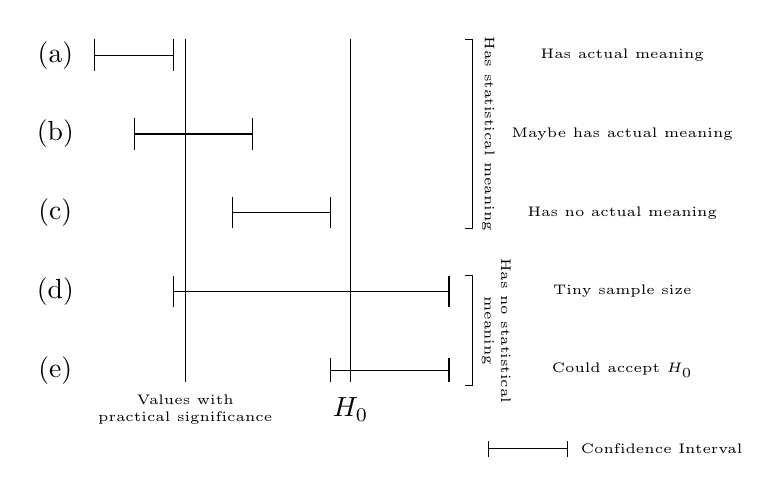
\begin{tikzpicture}
% Horizontal lines with error bars
\draw (0,5) -- (1,5); % Line a
\draw (0, 4.8) -- (0, 5.2); % Error bar for line a
\draw (1, 4.8) -- (1, 5.2); % Error bar for line a

\draw (0.5,4) -- (2,4); % Line b
\draw (0.5, 3.8) -- (0.5, 4.2); % Error bar for line b
\draw (2, 3.8) -- (2, 4.2); % Error bar for line b

\draw (1.75,3) -- (3,3); % Line c
\draw (1.75, 2.8) -- (1.75, 3.2); % Error bar for line c
\draw (3, 2.8) -- (3, 3.2); % Error bar for line c

\draw (1,2) -- (4.5,2); % Line d
\draw (1, 1.8) -- (1, 2.2); % Error bar for line d
\draw (4.5, 1.8) -- (4.5, 2.2); % Error bar for line d

\draw (3,1) -- (4.5,1); % Line e
\draw (3, 0.85) -- (3, 1.15); % Error bar for line e
\draw (4.5, 0.85) -- (4.5, 1.15); % Error bar for line e

\draw (1.15, 0.85) -- (1.15, 5.2); % first bar
\draw (3.25, 0.85) -- (3.25, 5.2); % second bar

% Labels for horizontal lines
\node at (-0.5,5) {(a)};
\node at (-0.5,4) {(b)};
\node at (-0.5,3) {(c)};
\node at (-0.5,2) {(d)};
\node at (-0.5,1) {(e)};

\node [font=\tiny, align=left] at (6.7, 5) {Has actual meaning};
\node [font=\tiny, align=left] at (6.7, 4) {Maybe has actual meaning};
\node [font=\tiny, align=left] at (6.7, 3) {Has no actual meaning};
\node [font=\tiny, align=left] at (6.7, 2) {Tiny sample size};
\node [font=\tiny, align=left] at (6.7, 1) {Could accept $H_0$};

% Vertical text on left
\node[rotate=270, font=\tiny] at (5,4) {Has statistical meaning};

\draw (4.8, 5.2) -- (4.8,2.8);
\draw (4.7, 2.8) -- (4.8,2.8);
\draw (4.7, 5.2) -- (4.8,5.2);

\node[rotate=270, font=\tiny, align=center] at (5.1,1.5) {Has no statistical \\ meaning};
\draw (4.8, 2.2) -- (4.8,0.8);
\draw (4.7, 0.8) -- (4.8,0.8);
\draw (4.7, 2.2) -- (4.8,2.2);


\draw (5,0) -- (6,0); 
\draw (5, -0.1) -- (5, 0.1);
\draw (6, -0.1) -- (6, 0.1); 
\node [font=\tiny, align=left] at (7.2, 0) {Confidence Interval};

% Text below the diagram
\node [font=\tiny, align=center] at (1.15, 0.5) {Values with \\ practical significance};
\node [align=center] at (3.25, 0.5) {$H_0$};

\end{tikzpicture}

\end{document}
